\documentclass[10pt,a4paper]{article}
\usepackage{amsmath}              
\usepackage{geometry}
\usepackage{amssymb}
\usepackage{graphicx}
\geometry{
a4paper,
total = {200mm,290mm},
left = 47mm,
right = 47mm,
top = 30mm,
bottom = 15mm,
}
\renewcommand{\baselinestretch}{1.1}

\usepackage[english]{babel} 
%\usepackage[pdftex]{graphicx}
\begin{document}
\begin{center}
\textbf{Head Count Compression Project Report 4}\\ 		%Title of the Report.
15th October,2015										%Date.
\end{center}
\begin{center}
\underline{\textbf{Objective}} \\
\end{center}	
$\bullet$ To build an application which enables us to compress an image using linear algebraic techniques and provide a count of the number of heads using image processing tools.
\begin{center}
\underline{\textbf{Choice of Tool}} 
\end{center}
$\bullet$ Matlab.\\
\begin{center}
\underline{\textbf{Image Color Models}} 
\end{center}
An Image can be in the following forms:\\
\textbf{Monochromatic}\\
The pixels are either represented in binary values 0 and 1 where 0 would be black and 1 would be white.
\\
\textbf{Gray Scale}
\\
8-bit gray scale image pixels can take values from 0 to 255 where 0 indicates absolute black and 255 indicates absolute black. Each pixel would require 8 bit for representation and hence gray scale image would require more memory than a binary image. There are again 2 bit and 3 bit gray scale images which primarily would have 4 and 8 levels of gray.\\
\textbf{Red Green Blue}\\
The pixels can be represented as the average of values of pixel values of three matrices, one representing all the shades of red, one for blue and one for green each ranging from 0 to 255. Generally an RGB image takes three times the space that a gray scale takes. Similarly, we can have 2 bit,3 bit, 6 bit  , 12 bit etc. that can represent 4,8,64, 4098… color respectively. Currently, 24 bit RGB model (True Color) is implemented that gives 16,777,216 colors.\\

To convert from a RGB to gray scale image the formula to be applied is:\\
 
Gray(x,y) = 0.299$\times$Red(x,y) + 0.587$\times$Green(x,y) + 0.114$\times$Blue(x,y)
\begin{center}
\underline{\textbf{Image File Formats}} 
\end{center}
\textbf{BMP(Bit Map)}\\
$\bullet$ The BMP format stores color data for each pixel in the image without any compression. For example, a 10$\times$10 pixel BMP image will include color data for 100 pixels. This method of storing image information allows for crisp, high-quality graphics, but also produces large file sizes.
It is an uncompressed format.\\
\textbf{GIF(Graphics Interchange Format)}\\
$\bullet$ The Graphics Interchange Format is the oldest graphic file format.  GIFs are 8-bit images, which limits them to a maximum of only 256 colors. GIFs use a lossless compression algorithm. LZW compression algorithm is used when an image is saved in the GIF format.\\
\textbf{PNG(Portable Network Graphics)}\\
$\bullet$ PNG is a lossless compression format.PNG has better compression than GIF and adds new features of its own,such as gamma storage,full alpha channel,true color support,and error detection.It also uses LZW compression.\\
\textbf{TIFF(Tagged Image File Format)}\\
$\bullet$ TIFF stands for Tagged Image File Format.TIFF images create very large file sizes.TIFF images are uncompressed and thus contain a lot of detailed image data(which is why the files are so big).\\
TIFF is the most common file type used in photo software such as Adobe Photoshop.\\
\textbf{JPEG(Joint Photographic Experts Group)}\\
$\bullet$ JPEG, is designed for compressing either full-color or gray-scale. JPEG is a lossy compression algorithm.  When you create a JPEG or convert an image from another format to a JPEG, you are asked to specify the quality of image you want and accordingly the image is compressed. More the compression, lower is the quality of the image.\\	
		
\begin{center}
    \begin{tabular}{ | l | l | l | p{5cm} |}
    \hline
    \textbf{Format} & \textbf{Compression Ratio} \\ \hline
    GIF & 4:1 - 10:1 \\ \hline
    JPEG(low to high Compression) & 10:1 to 100:1\\ \hline
    PNG & 20:1 \\
    \hline
    TIFF & 1:1\\
    \hline
    \end{tabular}
\end{center}

\begin{center}
\underline{\textbf{Representation Of Image as a Matrix}}\\
\end{center}
$\bullet$ Each pixel of an image is assigned with a value. An image hence can be represented as a two dimensional array (matrix) of values ranging from 0 to 255 in each case each value representing the value of the corresponding shade in RGB.The image itself is in continuous time domain and we are converting it in to discrete time domain with the help of sampling process.\\
$\bullet$ In Java, image can be converted into a two dimensional matrix by using a built in class of Raster. Firstly, file is imported into the program, where it I stored in an image file variable initialized with null. The width and height of the image is obtained with in-built function. A two dimensional array is declared and value of pixels is fetched and stored with the help of nested loops. The resulting 2-D array is the matrix representation of the image. 
\begin{center}
\underline{\textbf{Image Processing Techniques}}\\
\end{center}
\textbf{Color Transformation:}\\
Color Transformation is basically required for conversion between color models such as RGB, CMYK, so as different devices can work in proper order together. Methods such as Characterization and Calibration are employed to perform the task.\\
\textbf{Noise Filter:}\\
1.Smoothing(Mean Filter):\\
The value of the individual pixels is replaced by the mean of the neighboring values.\\
2.Median Filter:\\
Here we replace the value of individual pixels by the median of the surrounding values.  The median is calculated by first sorting all the pixel values from the surrounding neighborhood into numerical order and then replacing the pixel being considered with the middle pixel value.\\
3.Sharpening:\\
The Unsharp filter is a simple  sharpening operator which derives its name from the fact that it  enhances edges via a procedure which subtracts an unsharp, or smoothed, version of an image from the original image. We can also do image sharpening using Laplacian.\\
\begin{center}
  g(x,y) = f(x,y) – fsmooth(x,y)\\
\end{center}
\textbf{Enchancement:}
Enhancement basically makes the picture more visible. This involves techniques to normalize, equalize, color enhance images and so on. Modern interventions such as Red-Eye Reduction techniques fall under enhancements.\\
\textbf{Convolution:}
The basic idea is that a window of some finite size and shape is scanned across the image. The output pixel value is the weighted sum of the input pixels within the window where the weights are the values of the filter assigned to every pixel of the window itself.  Convolution of an image is done for smoothening or sharpening of the image.\\
\textbf{Mathematical Processes:}
This involves addition, subtraction, dilation(), erosion( The basic effect of the operator on a binary image is to erode away the boundaries of regions of foreground pixels ) and scalar multiplication.\\
\textbf{Edge Detection:}
It is a mathematical technique to highlight points where color brightness or shades change drastically. It can be done by the use of gradient or Laplacian of Gaussian edge detector on the image.\\
\textbf{Image analysis:}
Image analysis is done to extract relevant information from the image. One such technique is Histogram equalization in which the image is represented in the form of a histogram and contrast is adjusted according to histogram.\\
\textbf{Pseudo Color Image Processing:}
Pseudo Color Image Processing consists of assigning colors different than the original colors of the images based on a specified criterion. A pseudo color image is derived from a gray scale image by mapping each intensity value to a color according to a table or function. Pseudo color is typically used when a single channel of data is available (e.g. temperature, elevation, soil composition etc.), in contrast to false color which is commonly used to display three channels of data.
\begin{center}
\underline{\textbf{Image Compression Techniques}} 
\end{center}
$\bullet$ Image Compression refers to the process of reducing the amount of data required to represent a given quantity of information. Image compression may lead to loss of smaller details of the object however retaining the major details that make the object distinct and recognizable. In our case, compression leads to increase in pixel size which may lead to formation of blocks, however the image as a whole would still retain its major details like heads in our case. There are two kinds of compression, Lossy(better compression)  and Lossless(lesser compression).
\begin{center}
\textbf{Lossless Compression}\\
\end{center}
In Lossless Compression the original image can be perfectly recovered form the compressed (encoded) image. Lossless compression is used when the decompressed data and the original data need to be nearly same and when loss of minor details may cause problems.\\ 
\textbf{Run length encoding:}\\ 
This technique replaces sequence of identical symbols by shorter symbols.  Each value is represented as the value and its corresponding count. This type of compression is useful when the same data is reiterated multiple times in a sequence.\\
\textbf{Huffman encoding:} \\
The symbols that occur more frequently are assigned a smaller number of bits while the symbol that occur less frequently are assigned are relatively larger number of bits. This technique uses Huffman Tree Data Structure.\\ 
\textbf{LZW coding:}\\ 
 It replaces string of characters with single code. It does not do any analysis of the incoming text instead it just adds every new string of characters it sees to a table of strings. Compression occurs when a single code is used instead of string of characters. It compresses a file into a smaller file using a table-based lookup algorithm\\
\textbf{Area coding:}\\
Area Coding is same as Run length encoding but the only difference is that in a run length encoding we have a 1D array and in area Coding we use a 2D array. The algorithms for area coding try to find rectangular regions with the same characteristics. These regions are in a coded in descriptive form as an element with two points and a certain structure.\\
\begin{center}
\textbf{Lossy Compression}
\end{center}
Lossy Compression allows a loss in the actual image data i.e. the original data can’t be restored after this type of compression. These compression techniques are cheaper that is they take less time and space.\\
\textbf{Transformation Coding:}\\
It is a technique which uses Discrete Cosine Trans- form and Discrete Fourier Transform. JPEG uses DCT as its compression technique. A general transform coding scheme involves subdividing an N x N image into smaller n x n blocks and performing a unitary transform on each sub image. What the transform does is decorelate the original signal, and this decorrelation generally results in the signal energy being redistributed among only a small set of transform coefficients.\\
\textbf{Vector Quantization:}\\
The basic idea in this technique is to develop a dictionary of fixed-size vectors, called code vectors. A vector is usually a block of pixel values. A given image is then partitioned into non-overlapping blocks called image vectors. So Sup- pose we have 1 2 3 4 5 6 7 8. To store this we will require 3 bits. We will consider values: 1 and 2 as 00, 3 and 4 as 01, 5 and 6 as 10, 7 and 8 as 11. Now, on applying vector quantization the numbers can be represented in just 2 bits.\\
\textbf{Fractal coding:}\\
Partition the image domain into blocks of size s×s. For each block, search the image to find a block of size 2s×2s that is very similar to the original block. Select the mapping functions such that H(Di) = Ri  for each i. Hence, the data of 2sx2s gets reduced to s$\times$s that is almost one fourth.
 
\begin{center}
\underline{\textbf{Technique for Foreground and Background Separation}}
\end{center}
This process is used to separate Object and the background from the image.First mean of the histogram values is been calculated.We take a zero matrix as the background matrix. Then each pixel value is been compared with the mean histogram value.If it is smaller than the mean value,the original value is been added to the background matrix and the mean value is updated with that value else the mean value is added to the matrix.S×S size window scans the background image.Each pixel value is been modified with the average of S×S pixel neighbors.Hence we obtain the background matrix.Foreground image can be obtained by subtracting background matrix from original image matrix.
\begin{center}
\underline{\textbf{Thresholding Algorithms}}
\end{center}
\textbf{Histogram Shape Based Methods:}\\
We define two constants T1 and T2 and correspondingly change the value.
If f(x, y) < T1 then f(x, y) = 255 else if T1 ≤ f(x, y) < T2 then f(x, y) = 128 else f(x,y) = 0 where f(x,y) is a pixel value.\\
\textbf{Clustering Based Methods:}\\
Here the gray-level samples are clustered in two parts as background and foreground (object), or alternately are modeled as a mixture of two Gaussians.\\ 
\textbf{Entropy-based methods:}\\
Result in algorithms that use the entropy of the foreground and background regions, the cross-entropy between the original and binary image, etc.\\
\textbf{Object Attribute Based methods:}\\
This method searches a measure of similarity between the gray level and the binary images, such as edge coincidence etc.\\
\textbf{Spatial methods:}\\
Uses higher-order probability distribution and/or correlation between pixels.\\ 
\textbf{Local methods:}\\
Adapt the threshold value on each pixel to the local image characteristics. In these methods, a different T is selected for each pixel in the image.\\ 
\textbf{Hysteresis:} \\
If there is no clear valley in the histogram of an image it means that there are several background pixels that have similar gray level value with object pixels and vice versa. If this type of thing may happen then the solution is Hysteresis which classifies an object as pixels above the high threshold and a background below the low threshold.\\
\begin{center}
 \underline{\textbf{Image Labeling}}\\
\end{center}
Connected components labeling scans an image and groups its pixels into components based on pixel connectivity i.e. all pixels in a connected component share similar pixel intensity values and are in some way connected with each other. Once all groups have been determined, each pixel is labeled with a gray level or a color (color labeling). Connected component labeling works by scanning an image, pixel-by-pixel (from top to bot- tom and left to right) in order to identify connected pixel regions, i.e. regions of adjacent pixels which share the same set of intensity values V. (For a binary image V=1; however, in a gray level image V will take on a range of values, for example: V=51, 52, 53, ..., 77, 78, 79, 80. However, for the following we assume binary input images and 8-connectivity (Neighborhood Concept). The connected components labeling operator scans the image by moving along a row until it comes to a point p for which V=1. When this is true, it examines the four neighbors of p which have already been encountered in the scan (i.e. the neighbors (i) to the left of p, (ii) above it, and (iii and iv) the two upper diagonal terms). Based on this information, the labeling of p occurs as follows: If all four neighbors are 0, assign a new label to p, else if only one neighbor has V=1, assign its label to p, else if more than one of the neighbors have V=1, assign one of the labels to p and make a note of the equivalences. After completing the scan, the equivalent label pairs are sorted into equivalence classes and a unique label is assigned to each class. As a final step, a second scan is made through the image, during which each label is replaced by the label assigned to its equivalence classes. For display, the labels might be different graylevels or colors.\\

\begin{center}
\underline{\textbf{Image Compression}} 
\end{center}
We have compressed the image using two algorithms.\\
\begin{center}
\textbf{SVD(Singular Value Decomposition)}
\end{center}
In SVD we first separated original matrix of image in its RGB matrices.Then all three of these matrices were decomposed in U, S and V matrices.S matrix is diagonal matrix which holds the energy of the image.The values on its diagonal are in decreasing order which means that the major part of energy is 
stored on the upper part of the diagonal.Some values in this S matrix are very small i.e. they hold less energy hence such values are neglected.And the corresponding vectors of the U matrix and the V matrix are also neglected.Then we multiply these U,S and V matrices to again form the red green and blue components.Then combining the red green and blue matrices we get the compressed image.The image formed by this matrix is our compressed image as some energy of each matrix is reduced and that data is lost but the data lost is not major as we have only neglected the smaller values of diagonal on S matrix.This is a lossy compression.\\
\textbf{\ \ \ \ \ \ \ \ \ \ \ Original Image: \ \ \ \ \ \ \ \ \ \ \ \ \ \ \ \ \ \ \ \ \ \ \ \ \ \ \ \ \ \ \ Taking 25 eigen value:}\\
\includegraphics[trim = 1mm 8mm 2mm 5mm, clip, width=7cm]{Image_1_SS_Class_Quiz.jpg}
\includegraphics[trim = 1mm 8mm 2mm 5mm, clip, width=7cm]{25.jpg}\\

\textbf{\ \ \ \ \ \ \ \ \ \ \ \ \ \ \ \ \ 1944 KB \ \ \ \ \ \ \ \ \  \ \ \ \ \ \ \ \ \ \ \ \ \ \ \ \ \ \ \ \ 580KB}\\
\textbf{\ \ \ \ \ \ \ \ \ \ \ Taking 50 eigen value: \ \ \ \ \ \ \ \ \ \ \ \ \ \ \ \ \ \ \ \ \ \ \ \ \ \ \ \ Taking 100 eigen value:}\\
\includegraphics[trim = 1mm 8mm 2mm 5mm, clip, width=7cm]{50.jpg}
\includegraphics[trim = 1mm 8mm 2mm 5mm, clip, width=7cm]{100.jpg}\\

\textbf{\ \ \ \ \ \ \ \ \ \ \ \ \ \ \ \ \ 660 KB \ \ \ \ \ \ \ \ \  \ \ \ \ \ \ \ \ \ \ \ \ \ \ \ \ \ \ \ \ 792KB}\\
\begin{center}
\textbf{Discrete Cosine Transform(DCT)}
\end{center}
The DCT works by separating images into parts of different frequencies. It is a lossy compression.In DCT the image is broken 8x8 blocks of pixels.Working from left to right, top to bottom, the DCT is applied to each block.Each block is compressed through quantization.The array of compressed blocks that constitute the image is stored in a drastically reduced amount of space.When desired, the image is reconstructed through decompression and it uses Inverse Discrete Cosine Transform.\\

\textbf{\ \ \ \ \ \ \ \ \ \ \ Original Image: \ \ \ \ \ \ \ \ \ \ \ \ \ \ \ \ \ \ \ \ \ \ \ \ \ \ \ \ DCT:}\\
\includegraphics[trim = 1mm 8mm 2mm 5mm, clip, width=7cm]{Image_1_SS_Class_Quiz.jpg}
\includegraphics[trim = 1mm 8mm 2mm 5mm, clip, width=7cm]{DCT.jpg}\\

\textbf{\ \ \ \ \ \ \ \ \ \ \ \ \ \ \ \ \ 1944 KB \ \ \ \ \ \ \ \ \  \ \ \ \ \ \ \ \ \ \ \ \ \ \ \ \ \ \ \ \ 586KB}\\

\begin{center}
\textbf{Mathematical Morphological Techniques}
\end{center}
Morphological image processing is a collection of non-linear operations related to the shape or morphology of features in an image.\\
Morphological operations rely only on the relative ordering of pixel values, not on their numerical values and therefore are especially suited to the processing of binary images.\\ 
Morphological techniques probe an image with a small shape or template called a 'structuring element'.\\ 
The structuring element is positioned at all possible locations in the image and it is compared with the corresponding neighbourhood of pixels.\\ 
Some operations test whether the element "fits" within the neighbourhood, while others test whether it "hits" or intersects the neighbourhood.
The structuring element is a small binary image, i.e. a small matrix of pixels, each with a value of zero or one\\
1.The matrix dimensions specify the size of the structuring element.\\
2.The pattern of ones and zeros specifies the shape of the structuring element.\\
3.An origin of the structuring element is usually one of its pixels, although generally the origin can be outside the structuring element.\\

\includegraphics[trim = 1mm 1mm 1mm 1mm, clip, width=10cm]{elements.PNG}\\
When a structuring element is placed in a binary image, each of its pixels is associated with the corresponding pixel of the neighbourhood under the structuring element. The structuring element is said to fit the image if, for each of its pixels set to 1, the corresponding image pixel is also 1. Similarly, a structuring element is said to hit, or intersect, an image if, at least for one of its pixels set to 1 the corresponding image pixel is also 1. 

\includegraphics[trim = 1mm 1mm 1mm 1mm, clip, width=10cm]{2.PNG}\\
There are different types of techniques used for Mathematical Morphology which mainly use to erase noise as well as detect objects.\\  
Basically for removing noise we use these Morphological techniques:\\
1.Erosion. \\
2.Dilation. \\
3.Opening.\\
4.Closing. \\
For Object Detection and for modifying the objects these techniques are used:\\    
5.Connected Component.\\
6.Region Filling.  \\
7.Hit and Miss. \\
8.Convex hull. \\
9.Thinning. \\
10.Skeletonization.\\
 
\begin{center}
\underline{\textbf{Niblack Method}}
\end{center}
Ni-Black is a local thresholding algorithm that adapts the threshold according to the local mean and the local standard deviation over a specific window size around each pixel location. The local threshold at any pixel (i, j) is calculated as:\\
\begin{center}
$T(i,j) = m(i,j) + k \times \sigma^{2}(i,j)$\\
\end{center}Where m(i,j) and σ² (i,j) are the local sample mean and variance, respectively. The size of the local region (window) is dependent upon the application. The value of the weight 'k' is used to control and adjust the effect of standard deviation due to objects features.\\
\begin{center}
\underline{\textbf{Segmentation}}
\end{center}
Image segmentation is the process of partitioning a digital image into multiple segments(sets of pixels, also known as super pixels).The goal of segmentation is to simplify and change the representation of an image into something that is more meaningful
and easier to analyze.Image segmentation is typically used to locate objects and boundaries (lines, curves, etc) in images.More precisely, image segmentation is the process of assigning
a label to every pixel in an image such that pixels with the same label share certain characteristics(color, intensity).Each of the pixels in a region are similar with respect to some characteristic or computed property, such as color, intensity and texture. Adjacent regions are significantly different with respect to the same characteristic(s). \\
\begin{center}
\textbf{Image Segmentation Techniques}
\end{center}
\textbf{Threshold based Segmentation:}\\Histogram thresholding and slicing techniques are used to segment the image.\\
\textbf{Edge based segmentation:} \\With this technique detected edges in an image are assumed to represent object boundaries and used to identify these objects.\\
\textbf{Region based segmentation:}\\ A region based technique starts in the middle of an object and then growing outward until it meets the object boundaries.\\
\textbf{Clustering techniques:} \\Clustering methods attempt to group together patterns that are similar in some sense means it will group similar characterized pixels into an object.\\
\textbf{Matching:\\}When we know what an object we wish to identify in an image looks like, we can use this knowledge to locate the object in an image.This approach to segmentation is
called matching.\\
\begin{center}
\underline{\textbf{Head Count Result}}
\end{center}
We are still not get a perfect output actually we get 65 counts in which there are 6 or 7 noise which have been detected because of the infrastructure of the class.But our algorithm works perfectly when there are some certain  conditions like there are are no objects which has same black color as well as which can have same radius.\\
We are still working to improve our algorithm.\\

\textbf{\ \ \ \ \ \ \ \ \ \ \ Head Count: \ \ \ \ \ \ \ \ \ \ \ \ \ \ \ Thresholded:}\\
\includegraphics[trim = 1mm 1mm 1mm 1mm, clip,
 width=5cm]{count.PNG}
\includegraphics[trim = 1mm 1mm 1mm 1mm, clip,
 width=5cm]{1.jpg}\\


\textbf{\ \ \ \ \ \ \ \ \ \ \ Dilated and Eroded: \ \ \ \ \ \ \ \ \ \ \ \ \ \ \ \ \ \ \ \ \ \ \ \ \ \ \ \ Head Count:}\\
\includegraphics[trim = 1mm 1mm 1mm 1mm, clip, width=7cm]{test_dialated_eroded.jpg}
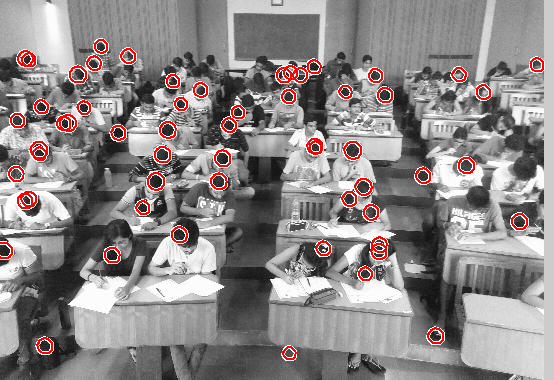
\includegraphics[trim = 1mm 1mm 1mm 1mm, clip, width=7cm]{final.PNG}\\
\\
\\
\\
\\
\\
\\
{\textbf{Flowchart of the WorkFlow:}\\
\\\
\includegraphics[trim = 1mm 1mm 1mm 1mm, clip, width=10cm]{flowchart.PNG}\\
\end{document}